% -*- TeX-master: "main"; fill-column: 72 -*-

\section{The Cell Behavior Ontology and the \token{cboTerm} attribute}
\label{sec:CBO}

It is difficult to determine the semantics of \Event constructs used to model intrinsic cellular behavior from SBML attributes alone. The \token{id} attribute on \Event objects allows for unique identification and cross-referencing while the \token{name} attribute allows the assignment of human readable labels to Events. Possible values for these attributes are unrestricted so that modelers can choose whichever fits their modeling framework and preference best. However, this means that without any additional human intervention, software tools are unable to discern the semantics of an extended \Event element modeling dynamic behavior. For instance, it would be inadvisable to interpret that an \Event is modeling the process of cellular death even if the \token{id} and \token{name} of such \Event have the \primtype{string} \val{Cell Death} as value. Additionally, as one may need to convert a dynamic \Event between different representations (e.g., Cellular Potts Model vs. Center-based off-lattice Model), there is a need to provide a standard, framework-independent, way of associating \Event components with given cellular processes.

A solution inspired by \sbmlthreecore is to associate model components with terms from carefully curated controlled vocabularies (CVs). This is the purpose of the \token{cboTerm} provided in the extended \Event class in \sec{subsec:extEvent}. The \token{cboTerm} facilitates the annotation of \Event components with terms belonging to the Cell Behavior Ontology (CBO) \citep{Sluka2014}. In this section, we discuss \textbf{CBO}, its usage in SBML models via the \token{cboTerm} attribute and relevant modeling implications.

\subsection{Cell Behavior Ontology (CBO)}
\label{subsec:bioCBO}

The development and use of bio-ontologies stems from the need to characterize and describe domains of biology in a standard way. The Cell Behavior Ontology (CBO) provides a carefully curated, controlled vocabulary that can be used to describe the behavior of a cell over time (dynamics) in a framework-independent manner, which enables the reliable exchange of biological descriptions. The Dynamic Structures SBML extension allows modelers to use a subset of the available identifiers to tag SBML \Event components via its attribute \token{cboTerm} to make the underlying biology and spatiality of the cellular process being modeled more explicit. The relationship between a \token{cboTerm} term describing an extended \Event and the CBO term being used is of the form "the Event is-A X", where X is the CBO term. Though CBO support provides an important source of information to understand the meaning of an \Event, software does not need to support cboTerms to be considered SBML-compliant.

The presence of a \token{cboTerm} attribute in an extended \Event is understood to change the way the \Event is interpreted and simulated. Annotating SBML \Event elements with CBO terms adds necessary semantic information that may also be used to convert such \Event from one framework to another when shared; it enables software tools to recognize precisely what cellular behavior this component is meant to model. For example, if the \token{cboTerm} has the value of \url{http://cbo.biocomplexity.indiana.edu/svn/cbo/trunk/CBO_1_0.owl#CellDeath} for a given \Event, regardless of the value that the \token{id} or \token{name} attributes are given or the modeling method used, the \Event labeled with this ontological term will be understood to model the dynamics of cellular death.

\subsubsection{Structure of the Cell Behavior Ontology}
\label{subsec:CBOstructure}

The purpose of CBO is to standardize the description of the intrinsic physical and biological characteristics of cells and tissues, which provides a basis for describing the spatial and observable dynamic behavior of cells in SBML models. To achieve this, CBO is split into controlled vocabularies for \textbf{CBO \textunderscore Objects}, which describe the physical entities of a biological model and \textbf{CBO \textunderscore Processs}, which describe the processes the aforementioned objects participate in. \ref{fig:CBOHierarchy} illustrates the taxonomy of CBO at the highest level.


\begin{figure}[tbhp]
	\centering
	%\usepackage{graphicx}
	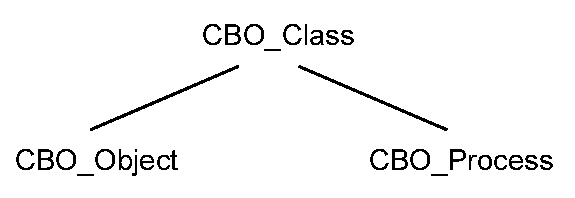
\includegraphics[width=0.25\textwidth]{images/CBO_Hierarchy.pdf}\\
	\caption{The controlled vocabularies that make up the main branches of CBO.} \label{fig:CBOHierarchy}
\end{figure}

As this SBML extension uses CBO only as a reference ontology for the description of dynamic processes described as events, all of the supported vocabulary is taken from the \textbf{CBO \textunderscore Process} branch. Though \textbf{CBO \textunderscore Process} terms encompass length scales that range from subcellular to cell aggregates and time scales that range from seconds to decades, only the subset in \sec{subsubsec:supportedCBO} is allowed.

\subsection{Using CBO and cboTerm}
\label{subsec:CBOTerm&CBO}

The \token{cboTerm} attribute for extended \Event constructs is always of \primtype{CBOTerm} data type, as defined in \sec{attr:cboTerm}. When present, the attribute's value must be the full identifier of a single term taken from the Cell Behavior Ontology (\url{http://bioportal.bioontology.org/ontologies/CBO}). The term chosen should be the most precise one that best summarizes the phenomenon represented by the extended \Event object. The relationship indicated by the presence of a non-empty \token{cboTerm} attribute in an \Event is of the form "the Event is-A X", where X is the CBO term. 

\subsubsection{Supported CBO terms in Event Components}
\label{subsubsec:supportedCBO}

One of the mechanisms the Dynamic Structures package uses to support the modeling of dynamic cellular behavior is the extension of the already existing SBML \Event construct. Under this extension, \Event objects carry a \token{cboTerm} attribute whose value must be a full term identifier, taken from the \textbf{CBO \textunderscore Process} vocabulary branch, which describes the behavior modeled by said \Event. Given substantial community input, the initial version of this package only supports a handful of dynamic cellular behaviors. \ref{fig:allowedCBO} displays supported dynamic processes and their corresponding CBO terms.

{\color{red} Harold: \notice I am being very conservative here. In consideration are growth and differentiation. Any other processes we wish this package to model?}

\begin{table}[h]
	\begin{tabular}{@{}ll@{}}
		\toprule
		\multicolumn{1}{c}{\textbf{Cell Behaviors}} & \multicolumn{1}{c}{\textbf{ CBO Terms}}                                   \\ \midrule
		Cell Division                              & http://cbo.biocomplexity.indiana.edu/svn/cbo/trunk/CBO\_1\_0.owl\#CellDivision        \\
		Cell Death                                 & http://cbo.biocomplexity.indiana.edu/svn/cbo/trunk/CBO\_1\_0.owl\#CellDeath           \\
		Cell Movement                       & 
		http://cbo.biocomplexity.indiana.edu/svn/cbo/trunk/CBO\_1\_0.owl\#Movement \\ \bottomrule
	\end{tabular}
		\caption{Supported cellular behaviors and corresponding CBO terms} \label{fig:allowedCBO}
\end{table}

We provide a description of each supported CBO term and of the expected simulation semantics given the constructs previously defined in \sec{sec:syntax}:

\begin{itemize}
	\item A \textbf{\textit{Cell Division}} term as value for the \token{cboTerm} attribute indicates that the \Event defines, by means of a \Trigger subobject, the mathematical conditions under which cellular division is to take place. When the \token{applyToAll} \Event attribute is set to \val{false}, the presence of this CBO term also dictates that model components whose \token{id} is referenced by an \Element in the \ListOfElements subobject have to be duplicated into a daughter cell. Quantities of the respective species and size of the compartments are set to half of the original in the case of symmetric cell division. When the value of \token{applyToAll} is val{true}, all model elements are duplicated. 
	
	\item A CBO term for \textbf{\textit{Cell Death}} as value for a \token{cboTerm} attribute indicates that the \Event defines, by means of a \Trigger subobject, the mathematical conditions under which cell death is to take place. When the \token{applyToAll} \Event attribute is set to \val{false}, the presence of this CBO term also dictates that SBML model components whose \token{id} is referenced by an \Element in the \ListOfElements subobject have to be removed from the model. When the value of \token{applyToAll} is val{true}, all model elements are removed. 	
	
	\item A CBO term for \textbf{\textit{Movement}} as value for a \token{cboTerm} attribute indicates that the \Event defines, by means of its \Trigger suboject, the mathematical conditions under which cell movement is to take place. When the \token{applyToAll} \Event attribute is set to \val{false}, the presence of this CBO term also dictates that SBML model \Compartments whose \token{id} is referenced by an \Element in the \ListOfElements subobject will have their position updated. When the value of \token{applyToAll} is val{true}, the spatial location of all model \Compartments is updated. 	

\end{itemize}

{\color{red} Should we include specific terms to support different kinds of cell division and cell death?}

\subsubsection{Tradeoffs in using CBO terms}
\label{subsec:tradeoffCBO}

The presented CBO-based approach to annotating SBML \Event components with controlled terms has, just like the SBO-based approach presented in \sbmlthreecore, the following strengths:

\begin{enumerate}
	\item The syntax required is very straight-forward and requires a single \primtype{string} containing the \primtype{id} of a supported CBO term.
	\item Supported CBO terms cover a relevant portion of the cellular behaviors required by the community.
	\item It does not interfere with already-existing annotation schemes implemented by either Core and SBML extensions.
\end{enumerate}

The following list illustrates some of the weaknesses of the proposed approach:

\begin{enumerate}
	\item The Cell Behavior Ontology is a recent and evolving ontology. As such, it is susceptible to minor changes in its hierarchical taxonomy. These however, should not affect the \token{ids} of the terms themselves but rather the structure of the ontology itself.
\end{enumerate}

{\color{red} Harold: \notice Can we think of any other benefits or weaknesses?}

\subsubsection{Relationships to the SBML annotation element}
\label{subsubsec:CBO&Annot}

A common mechanism used to provide information regarding modeled dynamic cellular behaviors is the \token{sBase} \Annotation component. Annotations are commonly used by software tools, which generally have their own vocabulary for supporting similar cellular behaviors. However, the best-practice recommendation for interoperability is to use the \token{cboTerm} attribute in the \Event object rather than an \Annotation component. Software tools are encouraged to translate their tool-specific \Annotation schemes to the proposed \textbf{CBO-based} approach when writing SBML models that include dynamic cellular behaviors.
